%%%%%%%%%%%%%%%%%%%%%%%%%%%%%%%%%%%%%%%%%%%%%%%%%%%%%%%%%%%%%%%%%%%%%%%%%%%%%%%%
%% Origin of this template:
%% https://authors.acm.org/proceedings/production-information

%% Commands for TeXCount
%TC:macro \cite [option:text,text]
%TC:macro \citep [option:text,text]
%TC:macro \citet [option:text,text]
%TC:envir table 0 1
%TC:envir table* 0 1
%TC:envir tabular [ignore] word
%TC:envir displaymath 0 word
%TC:envir math 0 word
%TC:envir comment 0 0

%% DOCUMENT CLASS %%%%%%%%%%%%%%%%%%%%%%%%%%%%%%%%%%%%%%%%%%%%%%%%%%%%%%%%%%%%%%
\documentclass[sigconf]{acmart}
% \documentclass[manuscript, screen, review]{acmart}


%% PACKAGES %%%%%%%%%%%%%%%%%%%%%%%%%%%%%%%%%%%%%%%%%%%%%%%%%%%%%%%%%%%%%%%%%%%%
\usepackage{csquotes}
\usepackage{fancyhdr}

%% SETTINGS %%%%%%%%%%%%%%%%%%%%%%%%%%%%%%%%%%%%%%%%%%%%%%%%%%%%%%%%%%%%%%%%%%%%

% Remove identation on "double-linebreaks".
\setlength{\parindent}{0pt}


%% LICENSE %%%%%%%%%%%%%%%%%%%%%%%%%%%%%%%%%%%%%%%%%%%%%%%%%%%%%%%%%%%%%%%%%%%%%

%% Remove all the licence, conference, ISBN and DOI information that are the
%% default for this template.
\settopmatter{printacmref=false} % Removes citation information below abstract
\settopmatter{printfolios=true} % Adds page numbers (optional, for review)
\renewcommand\footnotetextcopyrightpermission[1]{} % Removes conference footnote

% TODO: How to remove the conference from the page header?
% \acmConference[ ]{ }{ }{ }

%% CITATION %%%%%%%%%%%%%%%%%%%%%%%%%%%%%%%%%%%%%%%%%%%%%%%%%%%%%%%%%%%%%%%%%%%%

%% The majority of ACM publications use numbered citations and references.
%% The command \citestyle{authoryear} switches to the "author year" style.
%%
%% If you are preparing content for an event sponsored by ACM SIGGRAPH, you must
%% use the "author year" style of citations and references.
%% Uncommenting the next command will enable that style.
% \citestyle{acmauthoryear}

%% BEGIN %%%%%%%%%%%%%%%%%%%%%%%%%%%%%%%%%%%%%%%%%%%%%%%%%%%%%%%%%%%%%%%%%%%%%%%
%% End of the preamble, start of the body of the document source.
\begin{document}

%% TITLE %%%%%%%%%%%%%%%%%%%%%%%%%%%%%%%%%%%%%%%%%%%%%%%%%%%%%%%%%%%%%%%%%%%%%%%
%% The "title" command has an optional parameter,
% \title{Genetic Algorithms for Timetabling: The current state of the art}
\title{Overview of Genetic Algorithms in Educational Timetabling}

%% AUTHORS %%%%%%%%%%%%%%%%%%%%%%%%%%%%%%%%%%%%%%%%%%%%%%%%%%%%%%%%%%%%%%%%%%%%%
\author{Luca Quaer}
\email{luca@quaer.net}

\affiliation{
  \institution{Wilhelm Büchner Hochschule}
  \city{Darmstadt}
  \state{Baden-Württemberg}
  \country{Germany}
}

%% DATES %%%%%%%%%%%%%%%%%%%%%%%%%%%%%%%%%%%%%%%%%%%%%%%%%%%%%%%%%%%%%%%%%%%%%%%
% \received{20 February 2007}
% \received[revised]{12 March 2009}
% \received[accepted]{5 June 2009}


%% ABSTRACT %%%%%%%%%%%%%%%%%%%%%%%%%%%%%%%%%%%%%%%%%%%%%%%%%%%%%%%%%%%%%%%%%%%%

%% The abstract is a short summary of the work to be presented in the
%% article.
\begin{abstract}
Todo!
\end{abstract}


%% KEYWORDS %%%%%%%%%%%%%%%%%%%%%%%%%%%%%%%%%%%%%%%%%%%%%%%%%%%%%%%%%%%%%%%%%%%%
%% Keywords. The author(s) should pick words that accurately describe
%% the work being presented. Separate the keywords with commas.
\keywords{Genetic Algorithms, Educational Timetabling, Metaheuristics}


%% TITLE %%%%%%%%%%%%%%%%%%%%%%%%%%%%%%%%%%%%%%%%%%%%%%%%%%%%%%%%%%%%%%%%%%%%%%%
\maketitle


%% CONTENT %%%%%%%%%%%%%%%%%%%%%%%%%%%%%%%%%%%%%%%%%%%%%%%%%%%%%%%%%%%%%%%%%%%%%

%% Introduction ------------------------------------------------------------- %%
\section{Introduction}
% What is educational timetabling
Educational timetabling involves creating schedules for educational
institutions such as schools, colleges, and universities.
The problem domain can be divided into the following three main problems
\cite{kingston2013educational,schaerf1999survey}:
High-School Timetabling (HTT), University Course Timetabling (CTT) and
University Examination Timetabling (ETT).
Although a clear distinction between these three problems is not always
possible, they generally differ significantly from one another
\cite{Beligiannis2009}.
However, each of these problems essentially is a resource allocation problem
with the goal of assigning classrooms, instructors, and students to specific
time slots for various courses or activities, ensuring that all constraints and
requirements are met.
This includes avoiding conflicts (e.g., a student being scheduled for two
classes at the same time), adhering to institutional policies, and maximizing
the efficient use of resources.

% Why is it complicated?
The difficulty in finding a valid and effective solution to such a problem
lies in meeting the diverse requirements of different stakeholders
(e.g. students, teachers, administration), multiple constraints and resolving
resource conflicts in a combinatorial complex solution space caused by the
numerous constraints.
Timetabling problems like these are therefore known to be NP-complete in their
general form, meaning that the difficulty of finding a solution increases
exponentially with the problem size, which in turn makes it impossible to find
a deterministic algorithm providing an acceptable solution in polynomial time
\cite{Beligiannis2009}.
%
% What are solutions to the problem?
One popular approach to addressing the complexity of timetabling problems is the
use of metaheuristic algorithms \cite{Beligiannis2009}.
This class of algorithms leverages a non-deterministic search approach which
compromises on finding an optimal solution in favor of better runtime
performance. Consequently, such algorithms are not guaranteed to find
the best solution for a given problem, but a near optimal one
\cite{Affenzeller2009}.
Despite this limitation, metaheuristic algorithms are widely used in educational
timetabling due to their ability to provide high-quality solutions within
a reasonable timeframe.
These algorithms can be broadly classified into two categories: single-solution
and population-based metaheuristics \cite{Katoch2021}.
Single-solution based algorithms use a single candidate solution and iteratively
improve it by using local search, but are prone to get stuck in local maxima
\cite{Katoch2021}.
Population-based metaheuristics on the other hand work on multiple candidate
solutions during the search process, avoiding the risk of getting stuck
in a local maximum by maintaining diversity among the solution candidates
\cite{Katoch2021}.
Popular single-solution based algorithms in the timetabling domain are
simulated annealing, local search and Tabu search
\cite{Ceschia2023, Katoch2021}.
Well-known population based metaheuristics are genetic algorithms, particle
swarm optimization and ant colony systems \cite{Beligiannis2009, Katoch2021}.

% Solving problems of such complexity in a practicable timeframe is therefore
% mostly done by using metaheuristic algorithms, which find solutions to
% optimization problems but are not guaranteed to find the best solution.
% Therefore, optimization algorithms trying to find (near) optimal solutions have
% been used as alternative methods of solving educational timetabling problems.
% Examples for such methods are local search and simulated annealing techniques
% as well as computational intelligence algorithms like genetic algorithms (GAs),
% Tabu Search, Ant Systems and other metaheuristic approaches
% \cite{Beligiannis2009}.

% The algorithm of interest; Why are GAs well suited for timetabling?
Among these methods, genetic algorithms are known for their versatility and
application in a variety of use cases with the need of searching for solutions
of a combinatorial problem in a large solution space.
Therefore, this paper specifically focuses on genetic algorithms and how they
are used in the domain of educational timetabling.

% What is a GA?
Genetic algorithms (abbr. \textit{GA}) are a heuristic search method inspired by
the process of natural selection in biological evolution and thus belong to
the group of evolutionary algorithms \cite{Katoch2021}. As mentioned previously,
genetic algorithms utilize a population based approach, meaning multiple
solution candidates are iteratively evolved through numerous generations
imitating the Darwinian theory of survival of the fittest \cite{Katoch2021}.

% Introduce structure here? Or better do this in the "Methods" chapter?


%% Methods ------------------------------------------------------------------ %%
\section{Methods}
Veröffentlichungen der jüngeren Vergangenheit, insbesondere Survey Paper in
diesem Feld, welche Lösungsansätze für educational timetabling behandeln,
zeigten, dass die Populatität von Populations-basierte Algorithmen
wie genetische Algorithmen abgenommen hat. Dadurch hat sich im Bereich der
genetischen Algorithmen eine Forschungslücke aufgetan.
Außerdem ist dies kein "starker Indikator" dafür, dass diese Art von Algorithmen
grundsätzlich nicht geeignet für Timetabling Probleme ist, denn in diesem
Umfeld werden oft einfach die Algorithmen angewand, mit denen die jeweilige
Forschungsgruppe bereits Erfahrung gesammelt hat.

Das Ziel dieser Arbeit ist, die bisherige Verwendung von genetischen Algorithmen
speziell im Bereich des Educational Timetablings aufzuzeigen und übersichtlich
darzustellen.
Grundlage dessen ist eine umfassende systematische Literaturrecherche die
durchgeführt wurde, um viele relevante Anwendungen von genetischen Algorithmen
in der Domäne des Edu. Timetabling zu finden und anhand wesentlicher
Eigenschaften einzuordnen.
Dabei wurde auf verschiedene wissenschaftliche Datenbanken wie IEEE Xplore,
ACM Digital Library, SpringerLink und Google Scholar zurückgegriffen.
Die Suchkriterien umfassten Schlüsselbegriffe wie "genetic algorithm",
"educational timetabling", "timetabling", "scheduling", "heuristic" and
"metaheuristic".
Es wurde darauf geachtet, dass vorzugsweise aktuelle Veröffentlichungen, jedoch
auch ältere, etablierte Studien und Paper berücksicktigt wurden, um einen
umfassenden Überblick über die Entwicklung und den Einsatz genetischer
Algorithmen in diesem Feld zu erhalten und keine bereits eingesetzten
Methoden aufgrund ihres Alters auszuschließen.
Hauptaugenmerk war nichts desto trotz die ausführliche Beschreibung des
Algorithmus, um dessen Eigenschaften möglichst ausführlich zu dokumentieren.
Dieses Kriterium ist in vielen Veröffentlichungen nicht gegeben, vor allem der
Algorithmus bewusst nicht veröffentlicht wurde und deshalb nur auf dessen
Ergebnisse eingegangen wird.

Die Gliederung der vorliegenden Arbeit ist wie folgt:
Zunächst werden die Grundlagen von genetischen Algorithmen und zusätzlich
ausgewählte erweiterte Konzepte behandelt. Diese Einführung dient der besseren
Einordnung der später vorgestellten Algorithmen und deren Eigenschaften.
Die vorgestellten Methoden sind und können nicht erschöpfend sein und das
breite Feld der genetischen Algorithmen vollumfänglich behandeln.

Danach werden die in der Literaturrecherche herausgesuchten Algorithmen
anhand eines morphologischen Kastens genannt und deren wesentliche
Eigenschaften erarbeitet.
Dies ermöglicht einerseits eine Übersicht über den aktuellen Stand der Forschung
bezüglich genetischer Algorithmen für Educational Timetabling und zeigt
zusätzlich neue Forschungsansätze und -möglichkeiten auf, welche sich durch
nicht verwendete Kombinationen aus den Eigenschaften der Algorithmen ergeben.
Durch die systematische Analyse und Darstellung im morphologischen Kasten sollen
Wissenschaftler und Praktiker inspiriert werden, innovative und effektive
Lösungsansätze zu entwickeln und bestehende Methoden weiterzuentwickeln.

Abschließend wird über übergeordnete Erkentnisse aus der Literaturrecherche
eine Aussicht auf den potentiellen Erfolg von genetischen Algorithen
in zukünftiger Forschung gegeben.


% This paper specifically focuses on the application of genetic algorithms
% in the domain of educational timetabling and not timetabling or scheduling
% problems in general.
% To accomplish this, a thorough search among recent and early publications on
% this topic has been conducted, to create a representative overview of the most
% important concepts of genetic search used in the field of timetabling.
% After an introduction of the basic and some advanced concepts of genetic
% algorithms, the research results will be visualized and discussed.

% Do I need to include "how" I found the papers?


%% Basic Concepts ----------------------------------------------------------- %%
\section{Basic Concepts}
Genetic algorithms are a type of search and optimization algorithm inspired
by the biological process of reproduction and natural selection and represent
one branch in the field of evolutionary computing \cite{goldberg1989, Carr2014}.

In the search for a solution to an optimization problem, the set of possible
solutions -- the so-called solution space -- must first be determined and made
comprehensible for an algorithm in form of a data structure, which is suitable
for representing a solution \cite{Affenzeller2009}.
This representation of the solution is also called \textit{encoding} and
contains the data of a possible solution to the problem to be solved.
In nature, this data is encoded on chromosomes. Similarly, in genetic algorithms
the possible solution in coded form is also called \textit{chromosome} or
\textit{individual} \cite{Affenzeller2009}.

In addition, genetic algorithms employ a population based search approach,
whereby instead of a single potential solution a whole set of solutions is
iteratively improved. Such a set of solutions is called \textit{population}
and consists of multiple chromosomes. The stages of iterative improvements
are called \textit{generations} \cite{Affenzeller2009}.

In order for the algorithm to optimize towards a desired solution, it is
necessary to have a measure in place to evaluate and compare the chromosomes.
This value referred to as \textit{fitness} and is provided by the
\textit{fitness function} (also called \textit{objective function})
\cite{Affenzeller2009}.

With these basic terms defined, the general process of genetic algorithms
can now be described as follows:
First, an \textit{initial population} must be created and the fitness of its
chromosomes must be evaluated \cite{Affenzeller2009}.
Pairs (or triples, quadruples, etc.) are then selected
(\textit{selection} phase) from this population in order to reproduce
(known as \textit{crossover}) \cite{Affenzeller2009}.
The resulting offspring may undergo one or more mutations
(\textit{mutation} phase) with a defined probability before the fitness of
these new chromosomes is determined (\textit{evaluation} phase)
\cite{Affenzeller2009}.
Based on certain criteria chromosomes from the current generation and their
offspring are now selected, to replace the population with a new one
(\textit{replacement} phase) \cite{Affenzeller2009}.
The result of this step is a new generation of chromosomes forming a new
(usually fitter) population \cite{Affenzeller2009}.
From this population, chromosomes are once again selected for reproduction,
starting the process all over again \cite{Affenzeller2009}.
The genetic algorithm could theoretically continue indefinitely according to
this pattern, with termination conditions serving as the only means of halting
the process \cite{Beligiannis2009}.
%
The forementioned phases of genetic algorithms will be explained in the
following chapters.

%%% Encoding %%%
\subsection{Encoding}
Genetic algorithms require two essential components: an encoding and
a fitness function \cite{Affenzeller2009}.
The encoding plays a pivotal role in the design of a genetic algorithm
\cite{Katoch2021}.
Its most significant property is that it can completely represent the solution
space of the problem at hand, thereby deriving the potential solution to the
problem from a given chromosome \cite{Affenzeller2009}.
Moreover, the encoding must be designed in consideration of the data
processing of other genetic algorithm components, such as the fitness function
and the crossover operator \cite{Affenzeller2009}.
The fitness function must calculate the fitness value based on this
representation of a solution candidate, and the crossover operator should
generate offspring that are as valid as possible \cite{Affenzeller2009}.
In particular, the latter aspect can often only be fulfilled by an adapted,
domain-specific representation \cite{Affenzeller2009}.
%
The following paragraphs present some well-known encodings.

\subsubsection{Binary Encoding}
Binary encoding is a method in which chromosomes are represented as strings
of binary digits, i.e. an array of 0s and 1s \cite{Katoch2021}.
Each unit of information (also called a \textit{gene}) corresponds to one binary
digit (\textit{bit}).
%
The main advantage of binary encoding is the ability to use common and
well-researched crossover and mutation operators \cite{Katoch2021}.
However, these strategies lead to invalid representations, which
would need to be repaired \cite{Beligiannis2009}. Such repair strategies are
used in practice but pose the risk of introducing too much genetic information
which is from neither of the parents \cite{Affenzeller2009,Beligiannis2009}.
%
Furthermore, utilizing this encoding requires converting solution candidates
into binary form \cite{Katoch2021}. Depending on the complexity of the problem
this might not be feasible and thus require a different encoding.

Other well-known encoding schemes are \textit{decimal} and \textit{hexadecimal}
encoding. They work analogous to binary encoding except for using decimal and
hexadecimal digits respectively \cite{Katoch2021}.

\subsubsection{Value Encoding}
Value encoding is similar to binary encoding, as it also represents chromosomes
as strings of values. In contrast to binary encoding, these values can be
floating point numbers, integers or characters \cite{Katoch2021}.
This encoding scheme is mainly used for finding the optimal weights in a
neural network \cite{Katoch2021}.

\subsubsection{Permutation Encoding}
The permutation encoding method is commonly used in ordering problems
\cite{Katoch2021}. Similar to the encodings mentioned before, a chromosome
is made up of an array of values, but as the name suggests, the position in
the array encodes the order of the values in the context of an ordering problem
\cite{Katoch2021,Affenzeller2009}. Given that the objects of the ordering
problem are unique, this implies that the values in the array are unique too
\cite{Affenzeller2009}.

\subsubsection{Matrix Encoding}
Matrix encoding is a technique used in genetic algorithms where solutions are
represented as matrices (two-dimensional arrays) rather than as one-dimensional
arrays. This encoding is particularly useful for problems that
naturally map to a two-dimensional structure, such as scheduling, graphs
(as adjacency matrix) layout design, or certain combinatorial problems
\cite{Affenzeller2009}.



%%% Fitness Function %%%
\subsection{Fitness Function}
\enquote{In genetic algorithms a fitness function assigns a score to each
individual in a population; this fitness value indicates the quality of the
solution represented by the individual} \cite{Affenzeller2009}.
\enquote{Evaluating the fitness function for each individual should be
relatively fast due to the number of times it will be invoked}
\cite{Affenzeller2009}.
Consequently, it is arguably the most crucial component of a genetic algorithm,
and it is the only chance to steer the process of genetic evolution in
accordance with the desired optimization intentions
\cite{Beligiannis2009,kinnear1994perspective}.
Especially in the context of constrained optimization problems with multiple
objectives (e.g. hard and soft constraints), the fitness function must be
carefully designed to convey the correct optimization target for solving the
problem at hand \cite{Beligiannis2009,Carr2014}.
Timetabling problems usually pose multiple objectives in form of hard and
soft constraints \cite{Beligiannis2009}. These differ in their severity:
hard constraints must be satisfied in order for the solution to represent a
valid timetable, soft constraints on the other hand must not be satisfied and
only contribute to the quality of the solution \cite{Beligiannis2009}.

As previously stated, the design of the fitness function heavily depends on the
employed encoding scheme. The encoded data of a solution candidate serves as
the input value utilized by the fitness function to calculate the fitness of a
chromosome \cite{Affenzeller2009}. Although there is no universal recipe for
designing fitness functions, because they are highly domain-specific,
there are some methods that can be used as a starting point.
A prevalent method is to utilize a weighted sum as the foundation of a
multi-objective fitness function. Furthermore, such a function can be enhanced
through the incorporation of a penalty function, which accounts for constraint
violations at a specific weight per constraint \cite{Beligiannis2009}.

% OPTIONAL: Another option for multi-objective GAs is a Pareto-based fitness
%           function \cite{Katoch2021}.


%%% Initial Population %%%
\subsection{Initial Population}
Once an appropriate encoding and a fitness function have been established,
the initial step in the actual execution of the algorithm is to generate an
initial population \cite{Affenzeller2009}.
The initial population can be generated in two ways: randomly or heuristically.
If the problem's difficulty lies not in finding valid solutions, but in finding
the optimal solution, then heuristic initialization may be a beneficial
approach, as it could facilitate the evolution of the population.
However, in cases where finding a valid solution is already a significant
challenge, heuristics are not a viable option. In such instances, the initial
population must be created randomly \cite{Affenzeller2009}.

\subsection{Selection}
In the selection phase of a genetic algorithm, chromosomes are selected for
mating (\textit{crossover}) \cite{Affenzeller2009}.
The prerequisite for this phase of the genetic algorithm is, that the
fitness of each chromosome in the population has been evaluated
\cite{Affenzeller2009}.
At present, the most commonly employed selection techniques are roulette wheel,
rank, tournament, Boltzmann, and stochastic universal sampling
\cite{Katoch2021}.
The following sections present a brief overview of selected methods.

\subsubsection{Roulette Wheel}
The roulette wheel selection method is also called proportional selection
and works by assigning each individual a probability for reproduction according
to its fitness relative to the whole population \cite{Affenzeller2009}.
The expected value of the $i$-th chromosome to be selected for reproduction
is therefore $p_i = \frac{f_i}{\overline{f}}$ with $f_i$ denoting the fitness
of the $i$-th chromosome and $\overline{f}$ representing the average fitness
of all individuals in the population \cite{Affenzeller2009}.
\enquote{Therefore, each individual of the population is represented by a
space proportional to its fitness}\cite{Affenzeller2009} on an imaginary
roulette wheel.
\enquote{This wheel is then rotated randomly to select specific solutions that
will participate in formation of the next generatoin}\cite{Katoch2021}.

\subsubsection{Rank Selection}
\enquote{Rank selection is the modified form of Roul-ette Wheel selection.
It utilizes the ranks instead of fitness value}.
See \cite{Affenzeller2009}.
A possible approach of realizing this selection method is by ordering the
individuals according to their fitness and add copies of individuals in a way
that the best individual receives a pre-determined multiple number of copies
the worst one receives \cite{Affenzeller2009}.

Using this selection strategy reduces the dominating effect of outstanding fit
individual, but in turn distorts the difference between similarly fit
individuals, which increases the selection pressure in stagnant populations
\cite{Affenzeller2009}.
Compared to Roulette Wheel selection it reduces the chances of premature
convergence towards a local optimum \cite{Katoch2021}.

\subsubsection{Tournament Selection}
There are numerous variants of this selection method \cite{Affenzeller2009}.
The most common one is $k$-tournament selection where $k$ individuals are
randomly selected from a population and the fittest individual of the selected
ones is considered for reproduction \cite{Affenzeller2009}.
By choosing the tournament size $k$ appropriately, the selection pressure
can be easily scaled \cite{Affenzeller2009}.

% \subsubsection{Bolzmann}
% See \cite{Katoch2021}.

% \subsubsection{Comparison of selection techniques}
% See table 3 in \cite{Katoch2021}

%%% Crossover %%%
\subsection{Crossover}
Crossover is the genetic operator which performs the actual mating of
individuals selected during the selection phase \cite{Beligiannis2009}.
Given the close relation between the encoding scheme and the crossover operator,
certain crossover operators may not be compatible with some encodings in context
of the problem at hand \cite{Affenzeller2009}.

\subsubsection{Single Point}
The single point crossover method cuts each parent chromosomes into a head and
tail section. For this a random position is chosen at which both chromosomes
are cut \cite{Affenzeller2009}.
For a chromosome using binary encoding for example, this translates to
splitting the array used to represent the chromosome into two sections.
The tail sections are then swapped producing two new individuals
\cite{Affenzeller2009}.

\subsubsection{Multiple Point}
Similar to the single point crossover method, the multipoint crossover
cuts the parent chromosomes into sections. In contrast to the single point
crossover, and as the name suggests, the multipoint crossover method
uses multiple random cuts instead of a single one
\cite{Affenzeller2009,Katoch2021}. 

\subsubsection{Uniform Crossover}
Uniform crossover uses a randomly generated crossover mask, which contains
information about what parent chromosome provides certain genes to the
offspring \cite{Affenzeller2009}. This information could for example be:
\enquote{the first and second gene (e.g. first and second value in the array)
are taken from the first parent, the third gene is taken from the second
parent}.
To yield two children from the crossover operation, the mask can be inverted.
This process is equal to randomly swapping genes (at the same position) between
the parents and taking the resulting chromosomes as offspring \cite{Katoch2021}.


\subsubsection{Partially matched crossover}
Partially matched crossover is the most commonly used crossover operator,
as it performs better than most of the other operators \cite{Katoch2021}.
This crossover technique works by randomly choosing a continuous part of genes
from one parent, and swapping it with the corresponding genes (at the same
position) from the other parent chromosome \cite{Katoch2021}.
The left out genes are simply copied to the offspring chromosomes, except of
genes with values which are contained in the parts that were swapped between
the parents. The swapped section of genes denotes a mapping which is used to
map these values to the offspring chromosomes instead of simply copying them
\cite{Katoch2021}.

\begin{figure}[h]
  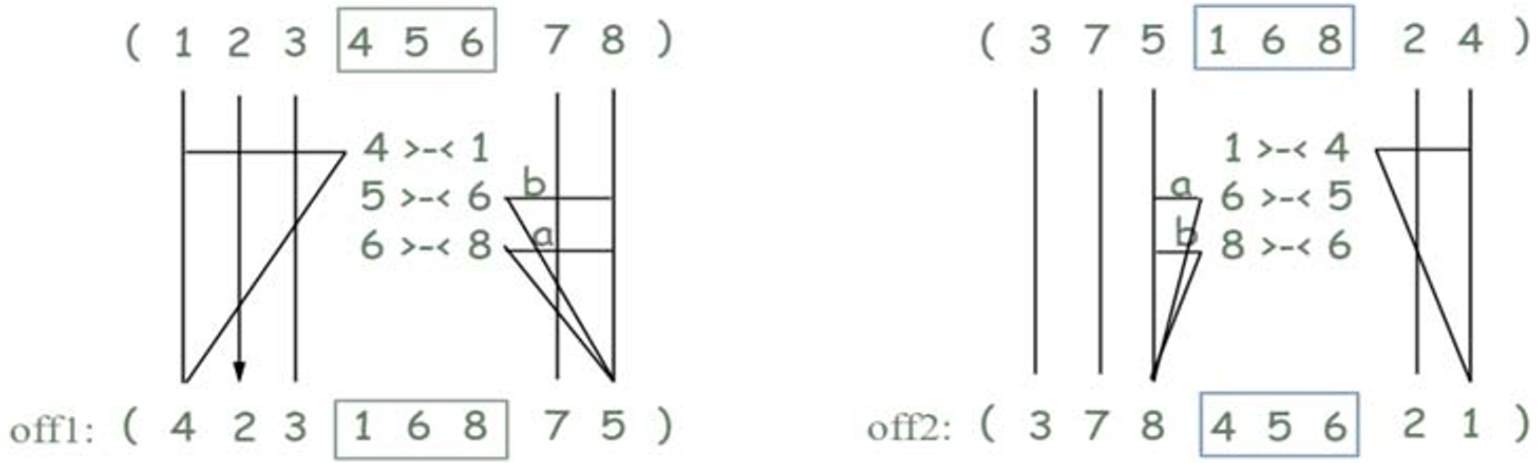
\includegraphics[scale=0.14]{assets/partially-matched-crossover.png}
  \caption{Partially matched crossover visualization \cite{Katoch2021}}
  \Description{Visualization of partially matched crossover operation}
\end{figure}


\subsubsection{Order crossover}
Order crossover copies one (or more) parts of the parent to the offspring
and fills the remaining space with genes from the respective present, which
are not present in the copied section \cite{Katoch2021}.

% \subsubsection{Shuffle crossover}
% See \cite{Katoch2021}.

% \subsubsection{Comparison of different crossover techniques}
% See table 4 \cite{Katoch2021}.

%%% Mutation %%%
\subsection{Mutation}
The mutation operator is used on the offspring created by the crossover
operation, to allow undirected jumps to slightly different areas of the search
space \cite{Affenzeller2009}. This procedure maintains genetic diversity
throughout generations and helps in efficiently exploring the search space
\cite{Katoch2021, Affenzeller2009}.

The actual implementation of the mutation operator greatly depends on the chosen
encoding, because mutating a chromosome could potentially lead to an invalid
solution candidate depending on how the encoding is designed.

Well-known mutation operators are displacement, simple inversion and scramble
mutation.

\subsubsection{Displacement Mutation (DM)}
The displacement mutation operator selects a random section from a chromosome
and moves it to another position on the chromosome \cite{Katoch2021}.
This operation does not change the sequence of the genes not included in the
moved section.

\subsubsection{Simple Inversion Mutation (SIM)}
For simple inversion mutation a random section is selected from a chromosome.
The order of the genes in this section is then reversed \cite{Katoch2021}.
This mutation can be further enhanced by also moving the section to another
position within the chromosome (similar to displacement mutation)
\cite{Katoch2021}.

\subsubsection{Scramble Mutation (SM)}
The scramble mutation is very similar to the simple inversion mutation with the
single difference of not inverting but shuffling the genes in the randomly
selected part of the chromosome \cite{Katoch2021}.


%%% Evaluation %%%
\subsection{Evaluation}
For the sake of completeness, the evaluation is listed here as separate phase,
even though this is not common in the researched literature. The evaluation
phase serves as the final step after successful application of the crossover
and mutation operations, in which the fitness of the new individuals
must be calculated in order to continue with the genetic algorithm.

%%% Replacement %%%
\subsection{Replacement}
After the current generation has reproduced in the selection, cross-over and
mutation phase, which created new offspring, the question arises as to which
of the new solution candidates should become members of the next generation
\cite{Affenzeller2009}. In context of evolution the replacement strategy
determines the life span of the individuals and substantially influences
the convergence behavior of the algorithm \cite{Affenzeller2009}.
The following schemes are possible replacement strategies for genetic
algorithms:

\subsubsection{Generational Replacement}
\cite{Affenzeller2009}
As the name already suggests, the generational replacement strategy simply
replaces the current population with the newly created offspring.
This process may result in a decrease of the fitness of the fittest individual
in the population at some stages of evolution \cite{Affenzeller2009}.

\subsubsection{Elitism}
With an elitism method of generation replacement, the best individual
(or the $n$ best individuals) of the previous generation are retained for
the next generation \cite{Affenzeller2009, Katoch2021}.
This theoretically allows individuals to be immortal and might lead to
premature convergence \cite{Affenzeller2009}.
The special case of only retaining the best individual is also called
\enquote{golden cage model} ($n$-elitism with $n = 1$) \cite{Affenzeller2009}.
In case the mutation operator is applied to the elite individuals to prevent
premature convergence, the replacement strategy is called \enquote{weak elitism}
\cite{Affenzeller2009}.

\subsubsection{Delete-$n$-last}
The $n$ weakest individuals are replaced by $n$ descendants
\cite{Affenzeller2009}. If $n$ is much smaller than the population size, this
strategy is known as steady-state replacement scheme \cite{Affenzeller2009}.
For $n = 1$, the changes between the old and new generations are minimal, while
choosing $n$ equal to the size of the population represents the previously
discussed generational replacement strategy \cite{Affenzeller2009}.


\subsubsection{Delete-$n$}
In contrast to the delete-n-last replacement strategy, this approach replaces
$n$ arbitrarily chosen individuals from the old generation rather than the
weakest ones \cite{Affenzeller2009}.
While this reduces the convergence speed of the algorithm, it also helps to
avoid premature convergence, balancing between elitism and weak elitism
\cite{Affenzeller2009}.

\subsubsection{Tournament Replacement}
Tournament replacement is similar to the equally named selection strategy.
In this replacement scheme competitions are run between sets of individuals
from the old population and their offspring \cite{Affenzeller2009}.
The winners of these tournaments become part of the new population
\cite{Affenzeller2009}.


%%% Termination %%%
\subsection{Termination}
As previously stated, the evolutionary process in genetic algorithms is
an infinite loop that requires a termination criterion to halt.
The desired termination constraint may vary depending on the problem and the
context in which the algorithm is used in.
One straightforward approach is to simply stop the genetic algorithm after a
certain number of generations has been reached \cite{Beligiannis2009}.
Another widely used method is to terminate the algorithm when the fitness value
of the best individual has not changed over a predefined number of
generations \cite{Carr2014}.


%% Advanced Techniques ------------------------------------------------------ %%
\section{Advanced Techniques}
In the field of genetic programming, it is common practice to adapt existing
methods to fit one's own use case. This has led to a steady development of new
approaches to improve genetic search in general.
While it is beyond the scope of this paper to provide an exhaustive overview
of the many branches of advanced genetic search,
the following sections present a selection of important in regard to solving
timetabling problems.

%%% Direct and Indirect Encoding %%%
\subsection{Direct and Indirect Encoding}
Genetic algorithms can be classified into two primary categories based on the
employed encoding scheme: \textit{direct} and \textit{indirect}
\cite{Thanh2007}.
In a direct encoding, the chromosome encodes all features of a solution
candidate, meaning that the whole search space is encoded
\cite{Thanh2007,Goos2002}.
Depending on the problem domain, this means, that chromosomes may also
represent invalid solution candidates. Therefore, direct encodings are prone
to hard constraint violations on crossover and mutation operations, which
requires applying additional mechanisms to find feasible solutions
\cite{Goos2002}.
One possible solution is to repair these invalid
chromosomes by applying a repair function that uses domain-specific
heuristics to transform the chromosome to a valid state, with the downside of
introducing genetic information not related to either of the parents
\cite{Beligiannis2009,Affenzeller2009}.

In contrast to a direct representation, an indirect (or \textit{implicit})
encoding only \textit{partially} encodes a solution candidate \cite{Thanh2007}.
One advantage of not encoding all information of a solution is, that
this restricts the search space the algorithm has to explore \cite{Goos2002}.
Furthermore, by using an indirect encoding, compliance with hard (and even
soft) constraints can be guaranteed, if the encoding is designed to
only represent valid solutions \cite{Goos2002}.

School timetabling problems are highly constrained, hence indirect
encodings have been successfully applied to such problems \cite{Goos2002}.


%%% Custom genetic operators %%%
\subsection{Custom genetic operators}
Especially for solving more complex solutions, like creating the forementioned
school timetable with many constraints, customized variants of genetic
operators may be necessary \cite{Beligiannis2009,Almeida2015}.
An example for such a custom operator is presented in \cite{Beligiannis2009}.
Their crossover operator is derived from a typical uniform crossover, but
it is adapted to the problem domain to not cause problems with a teacher's
schedule \cite{Beligiannis2009}.
Another potential application of such custom genetic operators could also be
the prevention of producing infeasible solutions, when using encoding schemes
that do not rule such invalid chromosomes out by design \cite{Elliman1995}.
%
Similarly to the custom crossover operator mentioned above,
mutation operators must also be adapted according to the chosen encoding
scheme \cite{Almeida2015}.

% \cite[8]{Affenzeller2009}
% You have to know what you do \cite{???}.


%%% Selection Pressure %%%
\subsection{Selection Pressure}
In the context of genetic algorithms, selection pressure refers to the
intensity with which the algorithm favors the fittest individuals during the
selection process for reproduction \cite{back1994selective, Affenzeller2009}.
%
When selection pressure is high, the algorithm strongly favors the best
individuals in the population. These individuals are more likely to be selected
for reproduction, leading to a quicker convergence towards optimal or
near-optimal solutions. However, if the pressure is too high, it might cause
premature convergence, where the population loses diversity and gets stuck in
local optima \cite{back1994selective}.

Conversely, when selection pressure is low, the algorithm less strongly favors
the fittest individuals. This allows for a more diverse set of individuals
to be selected for crossover. This helps to maintain genetic diversity within
the population and can avoid premature convergence. However, if the pressure
is too low, the algorithm may converge very slowly or struggle to find optimal
solutions efficiently \cite{back1994selective}.

Consequently, the selection pressure generated by the utilized selection method
is always a compromise between convergence speed and avoiding premature
convergence. It appears, that a dynamic intervention in the evolutionary process
to adapt the selection process and the associated selection pressure would
result in an improvement of the algorithm. This is exactly the approach taken
by the offspring selection method explained in the following paragraph.


%%% Offspring Selection (OS) %%%
\subsection{Offspring Selection}
Offspring selection (OS) is a self-adaptive selection pressure steering method
\cite{Affenzeller2009}.
Contrary to what the name suggests, this method does not replace previously
presented selection methods, such as roulette-wheel or linear-rank schemes.
Instead, a second selection step is introduced \cite{Affenzeller2009}.
After the first selection step has been executed (for example roulette-wheel
selection) and the crossover operation has been applied to the selected
chromosomes, a further selection -- the offspring selection -- is applied
\cite{Affenzeller2009}.

The offspring selection considers the fitness of the individuals resulting from
crossover.
To assure the genetic search mainly progresses with successful offspring,
the newly introduced selection step guarantees that a sufficient number of
children surpass their parents' fitness \cite{Affenzeller2009}.
The success ratio ($SuccRatio \in [0, 1]$) controls the proportion of
individuals in the next generation, with better fitness than their parents
\cite{Affenzeller2009}.

This inevitably leads to the following question:
\enquote{Is a child better than its parents, if it surpasses the fitness of the
weaker parent, the better parent, or some kind of weighted average of both?}
\cite{Affenzeller2009}.
To answer this question the offspring selection method introduces a comparison
factor ($CompFactor \in [0, 1]$), inspired by simulated annealing. This factor
sets a fitness threshold between the worse and better parent. Early in the
process, offspring only need to surpass the fitness of the weaker parent to
be considered \textit{better}. As the algorithm progresses, this threshold
increases towards the fitness of the better parent, facilitating a broader
search initially and a more focused search later \cite{Affenzeller2009}.
% affenzeller s.70
The gradual increase of the comparison factor adjusts the selection pressure
throughout the genetic search process, starting with a low selection pressure
to prevent premature convergence and steadily increasing the pressure to
not suffer from long runtimes until the search converges \cite{Affenzeller2009}.


%%% Parallel Genetic Algorithms %%%
\subsection{Parallel Genetic Algorithms}
Genetic algorithms are well suited for parallelization. There are various
methods of implementing these, some of which require fundamental changes to the
algorithm and others do not \cite{Affenzeller2009}.
%
Concepts for parallel genetic algorithms fall into three categories:
global parallelization, coarse-grained parallel GAs and fine-grained parallel
GAs. The most popular for practical applications is the coarse-grained model,
also known as the island model \cite{Affenzeller2009}.

\subsubsection*{Global Parallelization}
In global parallelization, a single population is used, and selection involves
all individuals. This method retains the same qualitative properties as a
sequential GA, with the primary parallelized operation being the evaluation of
individual fitness. A master node distributes and collects workloads from slave
processors, making this model efficient when fitness evaluation is the primary
runtime bottleneck \cite{Affenzeller2009}.
\begin{figure}[h]
  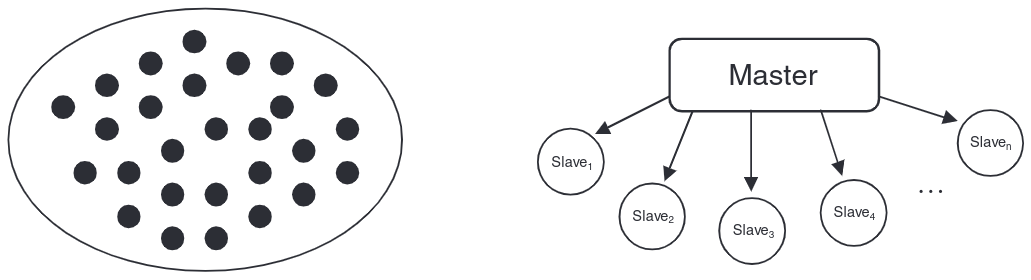
\includegraphics[scale=0.22]{assets/parallel-ga-global.png}
  \caption{
    Global parallelization: Single population (left) and the corresponding
    master-slave model (right) \cite{Affenzeller2009}.
  }
  \Description{Visualization of global parallelization concept}
\end{figure}

\subsubsection*{Coarse-grained parallel genetic algorithms}
Coarse-grained parallel GAs divide the population into subpopulations
(called \textit{islands} or \textit{demes}) that evolve mostly in isolation,
occasionally exchanging individuals during migration phases.
This model introduces significant changes to the algorithm structure,
differing from sequential genetic algorithms \cite{Affenzeller2009}.
The main idea is that isolated demes will converge to different regions of the
solution space, with migration and recombination combining relevant solution
parts \cite{Affenzeller2009}.
Coarse-grained parallel genetic algorithms are widely used due to their
ease of implementation and therefore the most popular method of
parallelizing genetic algorithms \cite{Affenzeller2009}.
\begin{figure}[h]
  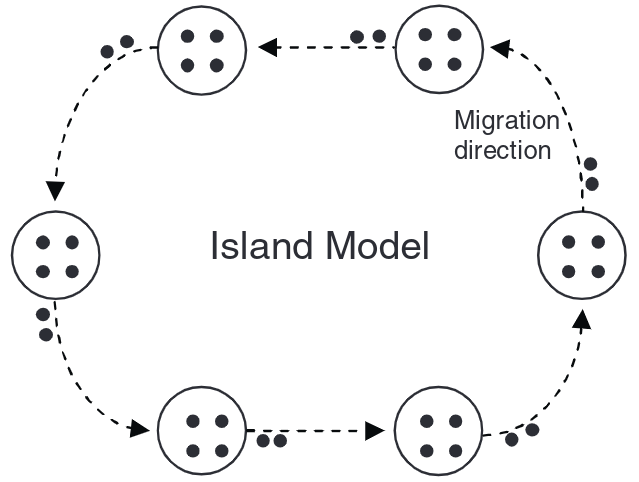
\includegraphics[scale=0.24]{assets/parallel-ga-coarse.png}
  \caption{
    Population structure of a coarse-grained parallel genetic algorithm
    \cite{Affenzeller2009}.
  }
  \Description{
    Visualization of the population structure in a coarse-grained parallel
    genetic algorithm
  }
\end{figure}

\subsubsection*{Fine-grained parallel genetic algorithms}
Fine-grained parallel genetic algorithms involve many small demes which are
part of one spatially distributed population \cite{Affenzeller2009}.
The idea behind this is that individuals are spread throughout the
global population like molecules in a diffusion process, with recombination
restricted to local neighborhoods \cite{Affenzeller2009}.
\begin{figure}[h]
  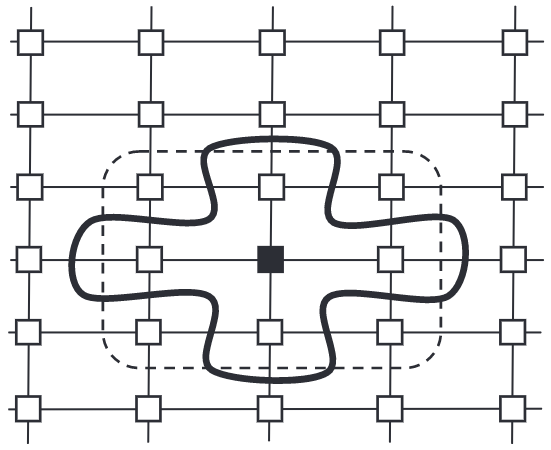
\includegraphics[scale=0.24]{assets/parallel-ga-fine.png}
  \caption{
    Population structure of a fine-grained parallel genetic algorithm
    with a cellular model \cite{Affenzeller2009}.
  }
  \Description{
    Visualization of the population structure in a fine-grained parallel
    genetic algorithm using a cellular model
  }
\end{figure}


%% Discussion --------------------------------------------------------------- %%
\section{Discussion}
In diesem Kapitel werden die Ergebnisse der systematischen Literaturanalyse
vorgestellt und diskutiert. Der Fokus liegt dabei auf der Darstellung der
verschiedenen genetischen Algorithmen und der Darstellung derer Eigenschaften
in einem morphologischen Kasten. Dabei wird untersucht, welche Kombinationen
von Eigenschaften bisher erfolgreich angewendet wurden, welche bis dato
weniger Aufmerksamkeit erfuhren und welche neuen Kombinationen Potenzial für
zukünftige Forschung bieten.

Die Tabelle xyz zeigt die im Rahmen der Literaturrecherche betrachteten
Algorithmen und deren wesentliche Charakteristika:
% Morphologischer Kasten -> hier einfügen

% Trends auswerten:
% - häufigste selektionsmethode
% - beliebtestes encoding
% - parallelität spielt kaum ein Thema -> birgt aber ein riesen potential (GPU)
  % potenzial der besseren parallelisierung ggü von populären integer
  % programming methoden. das könnte der game changer sein % gerade bei
  % parallelisierung mit GPUs

% - Der morphologische Kasten identifiziert verschiedene Kombinationen von
  % Eigenschaften, die bisher wenig oder gar nicht untersucht wurden.
  % Insbesondere die Kombination von adaptiven Selektionsmethoden mit
  % fortschrittlichen Mutationsmechanismen bietet ein großes Potenzial für
  % zukünftige Forschungen. Diese neuen Ansätze könnten zu effizienteren und
  % effektiveren Lösungen für das educational timetabling führen.
  %
  % +++ und PARALLELISIERUNG !!!

% - Untersuchung der Auswirkung weiterer parameter (Mutationswarhscheinlichkeit
%   usw. auf den Selection Pressure)


%% Conclusion --------------------------------------------------------------- %%
\section{Conclusion}
To do.

%% Future Work -------------------------------------------------------------- %%
\section{Future Work}
The findings from this work will serve as the basis for the author's master's
thesis, in which a genetic algorithm for a special timetabling problem will be
developed.
The examinations conducted in this paper provide information about the most
frequently used techniques of genetic search within the timetabling domain,
which will serve as a reference point for selecting the most appropriate
genetic methods for the algorithm to be developed.


%% ACKNOWLEDGEMENTS %%%%%%%%%%%%%%%%%%%%%%%%%%%%%%%%%%%%%%%%%%%%%%%%%%%%%%%%%%%%
% \begin{acks}
% To Robert, for the bagels and explaining CMYK and color spaces.
% \end{acks}

%% BIBLIOGRAPHY %%%%%%%%%%%%%%%%%%%%%%%%%%%%%%%%%%%%%%%%%%%%%%%%%%%%%%%%%%%%%%%%
\bibliographystyle{ACM-Reference-Format}
\bibliography{main}


%% APPENDIX %%%%%%%%%%%%%%%%%%%%%%%%%%%%%%%%%%%%%%%%%%%%%%%%%%%%%%%%%%%%%%%%%%%%
% \appendix
% \section{Research Methods}


%% END %%%%%%%%%%%%%%%%%%%%%%%%%%%%%%%%%%%%%%%%%%%%%%%%%%%%%%%%%%%%%%%%%%%%%%%%%

\end{document}
\endinput

%%%%%%%%%%%%%%%%%%%%%%%%%%%%%%%%%%%%%%%%%%%%%%%%%%%%%%%%%%%%%%%%%%%%%%%%%%%%%%%%
